%!TEX root = ../../Main.tex
\graphicspath{{Chapters/Indledning/}}
%-------------------------------------------------------------------------------

\chapter{Indledning}
\section{Indledning}
Under optagelse til et live madprogram, sker det ofte at værten skal bruge en blender/foodprocesser. Dette betyder at værten ikke kan kommunikere med seerne mens blenderen/foodprocesseren kører. Denne problematik vil Noise Suppression System (NSS) kunne afhjælpe. Gennem en digital signal prossesering (DSP), vil vi dæmpe støjsignalet fra en køkkenmaskine dynamisk i realtid. Systemet består af to mikrofoner, et placeres tæt på støjen, et andet tæt på værten. De to mikrofoner fungere som input til vores system (Blackfin), hvor procceseringen og filtreringen foregår. Efter proceseringen bliver produktet afspillet på en højtaler, som erstatning for højtaleren fra et tv-apperat. Et overblik over systemet kan ses på figur \ref{fig:konceptbillede}

\begin{figure}[H]
	\centering
	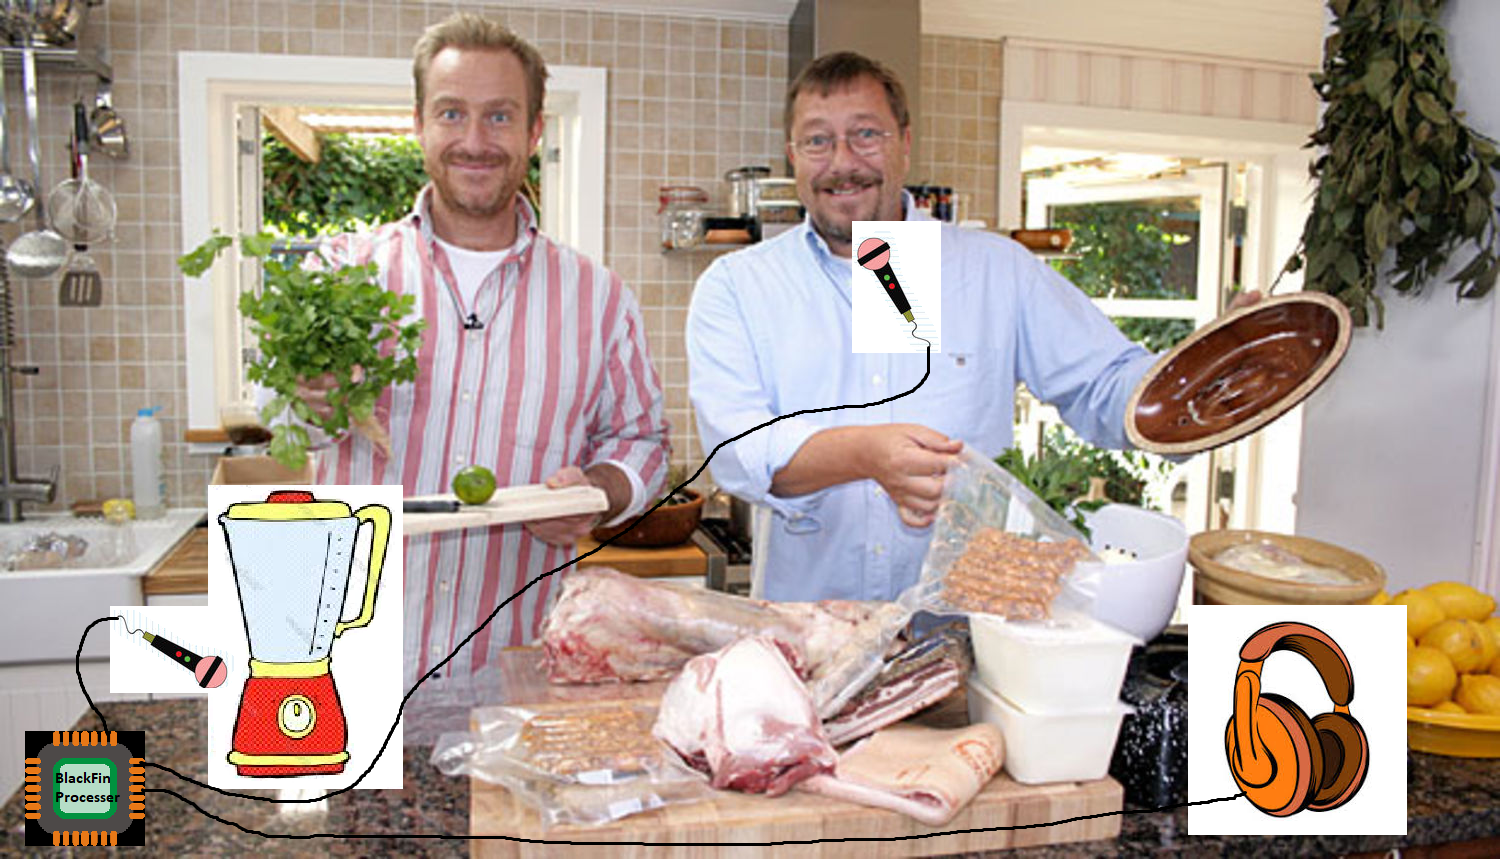
\includegraphics[width = 400pt]{Img/Konceptbillede}
	\caption{Konceptbillede for NSS}
	\label{fig:konceptbillede}
\end{figure}

Med udgangspunkt i brugerens behov vil der blive opstillet en række brugsscenarier, der beskriver brugerens interaktion med systemet. Disse scenarier vil sammen med en række veldefinerede krav og afgrænsninger, danne grundlaget for designet af alle dele af systemet.  \\ 

\newpage

\section{Teori}
I procceseringsfasen af projektet, har vi valgt at bruge et adaptivt filter - LMS (Least Mean square) algoritme. Et adaptivt filter består af 2 funktionelle blokke, hvor den ene blok fungerer som et filter, fra dynamiske kofficienter som bliver opdateret LMS blokken.  Filteret trækker herefter de beregnede filter fra det samlede lydsignal. 
   

\begin{figure}[H]
	\centering
	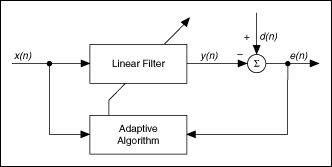
\includegraphics[width = 400pt]{Img/Figures}
	\caption{LMS adaptive filter}
	\label{fig:LMS_filter}
\end{figure}

På figur \ref{fig:LMS_filter} ses et overblik over det adative system, hvor x(n) er støjsignalet, y(n) er det filtrede støjsignal, med koefficienter som opdateres fra blokken "Adaptive Algoritm". d(n) er det ønskede signal inklusiv det støjende signal. e(n) er forskellen mellem d(n) og y(n) og derved støjen fratrukket fra det samlede signal af ønsket og støj.  